\documentclass[onecolumn, hmargin=1in, vmargin=1in]{aastex62}
%%%%%%begin preamble
%\usepackage[hmargin=1in, vmargin=1in]{geometry} % Margins
\usepackage{hyperref}
\usepackage{url}
\usepackage{natbib}
\setlength{\bibsep}{0pt plus 0.3ex}
\usepackage{graphicx}
\usepackage{amsmath}
\usepackage{amsfonts}
\usepackage{amssymb}

\usepackage{color}
\hypersetup{
  colorlinks   = true,
  %citecolor    = blue
  citecolor    = gray
  % gray is not being found!?!
  % gray is found if pdfpages is used... crap.
  %citecolor    = grey
  %citecolor    = Gray
}

%% headers
\usepackage{fancyhdr}
\pagestyle{fancyplain}
\fancyhf{} % sets both header and footer to nothing
\lhead{Evan Anders -- Research Statement}
\rhead{Princeton Dept.~Astrophysical Sciences Postdoctoral Research}
\cfoot{\footnotesize{\thepage}}

\renewcommand{\vec}{\ensuremath{\boldsymbol}}
\newcommand{\dedalus}{\href{http://dedalus-project.org}{Dedalus}}
\newcommand{\del}{\ensuremath{\vec{\nabla}}}
\newcommand{\scrS}{\ensuremath{\mathcal{S}}}

\newcommand{\prf}{Physical Review Fluids}


\begin{document}
Main sequence stars with masses similar to the Sun rely on vigorous near-surface convective regions to transport their stellar luminosity.
Helioseismology and asteroseismology measure the surface signatures of waves launched by these convective motions to examine the interior of the Sun and other stars.
Asteroseismic measurements have precisely determined the mass and radius of many stars and are used broadly across astrophysical disciplines including exoplanetary science and galactic archaeology \citep{huber&all2019}.

Interpretation of asteroseismic data requires one-dimensional (1D) stellar structure models. 
State-of-the-art codes like MESA \citep{paxton&all2011} which generate 1D stellar structure profiles have known deficiencies \citep{buldgen2019}, including their reliance on parameterizations of convection like mixing length theory \citep[MLT,][]{bohm-vitense1958}.
MLT predicts that large-scale ``giant cells'' should be driven in the deep convection zone of solar-type stars.
Unfortunately, modern helioseismic observations and direct measurements of flows on the Sun's surface have not detected giant cells \citep{hanasoge&all2015, hathaway&all2015}.
The absence of these flows has called into question our most fundamental understanding of the nature of convection in stars, a problem widely referred to as the ``Solar Convective Conundrum.''
Improving our understanding of convection, and thus improving stellar structure models, is critical to improving asteroseismic observations.
In my research, I create and study numerical simulations using the Dedalus pseudospectral framework \citep{burns&all2019} with the goal of solving this Convective Conundrum.

\vspace{-44pt}
\section*{\textbf{Past \& Current Results: Fundamental Studies in Stellar Convection}}
\thispagestyle{fancy}
\paragraph{Scaling Laws in Fully Compressible, Stratified Convection}
Modern computational resources cannot create simulations which achieve the same levels of turbulence as stellar convection \citep{brummell&all2002}.
Modern convection research therefore tends to study how convective properties like the efficiency of heat transport scale with increased convective driving and attempt to extrapolate out to stellar parameters.
In \citet{anders&brown2017}, we determined how to straightforwardly set the Mach number of fully compressible, stratified convection, and learned that scaling laws in both low- and high-Mach number convection are almost identical to those seen in incompressible convection \citep{ahlers&all2009}.
In \citet{anders&all2019}, we built on this work by adding rotation to these fully compressible convective studies.
We demonstrated a procedure for specifying the degree of rotational constraint felt by the convective flows \emph{a priori}, which had not been done in previous studies.
When the degree of rotational constraint was specified and convective driving was increased, we found the same incompressible scaling laws emerge.
I am currently extending these studies by collaborating with Dr.~Nick Featherstone (Univ.~Colorado) to determine if the degree of rotational constraint can be specified \emph{a priori} in simulations which employ spherical geometries.

\paragraph{Accelerated Evolution of Convective Simulations}
Modern simulations of stellar convection generally include a transient phase during which the thermodynamic structure of the domain is relaxing into an equilibrium state.
As simulations are pushed into highly-turbulent, more astrophysically-interesting regimes, this relaxation timescale becomes very long compared to the overturn timescale of convective dynamics.
In state-of-the-art simulations, before meaningful measurements can be taken, this timescale separation creates a long period of rundown which is physically uninteresting and very computationally expensive to timestep through.
In \citet{anders&all2018}, we found a mechanism for fast-forwarding through this equilibration time in a very simple convective system, and verified that it produced the same results to within 1\% of standard timestepping techniques using an order of magnitude fewer cpu-hours.

I am currently working with Prof.~Geoff Vasil (Univ.~Sydney) to demonstrate the importance of achieving thermally equilibrated solutions, particularly when complications like rotation are included.
We have found that within a single simulation of convection, the amount of influence that rotation exerts over convective flows can change by an order of magnitude in the equilibrated state compared to at early times, and will publish these results in the Spring.

\paragraph{Entropy Rain: Thermals in Stratified Domains}
Stratified convection, like that in the envelopes of solar-type stars, exhibits asymmetrical flows: upwellings are slow, weak, and wide while downflows are intense, fast, and narrow.
The ``entropy rain'' hypothesis posits that downflows may be so powerful in stellar envelope convection that they alone transport the stellar luminosity, and upflows exist only to conserve mass while transporting negligible energy.
This idea is gaining traction, and could explain the absence of giant cells in observations \citep{hanasoge&all2015}.
A schematic of the entropy rain picture is shown in Fig.~\ref{fig:tri_panel}a.
It is possible these downflows turbulently break up into distinct pieces as they fall and these individual downflow pieces can be modeled as ``thermals.''
Thermals are regions of cold fluid which accelerate due to buoyancy forces and shape themselves into vortex rings; an evolved turbulent thermal is visualized in Fig. \ref{fig:tri_panel}b.
Thermals are also observed and studied in the Earth's atmosphere \citep{lecoanet&jeevanjee2019}.

In \citet{andersLB2019}, we studied how an atmospheric density stratification affects the size of thermals as they propagate.
We found that thermals compress less than a simple estimate based on the stratification alone would anticipate \citep{brandenburg2016}.
We further estimated to our surprise that thermal-like downflows could very easily carry the Sun's luminosity through much of the solar convection zone, in agreement with the entropy rain hypothesis.
I am currently extending this work with Prof.~Daniel Lecoanet (Princeton / Northwestern) and Dr.~Lydia Korre (Univ.~Colorado) to understand how thermals behave when they impinge upon the stable radiative zone at the base of a stellar envelope convection zone.

\section*{\textbf{Proposed Research: Stellar Convection Across Spatial Scales}} 
\begin{figure*}[t]
	\begin{center}
    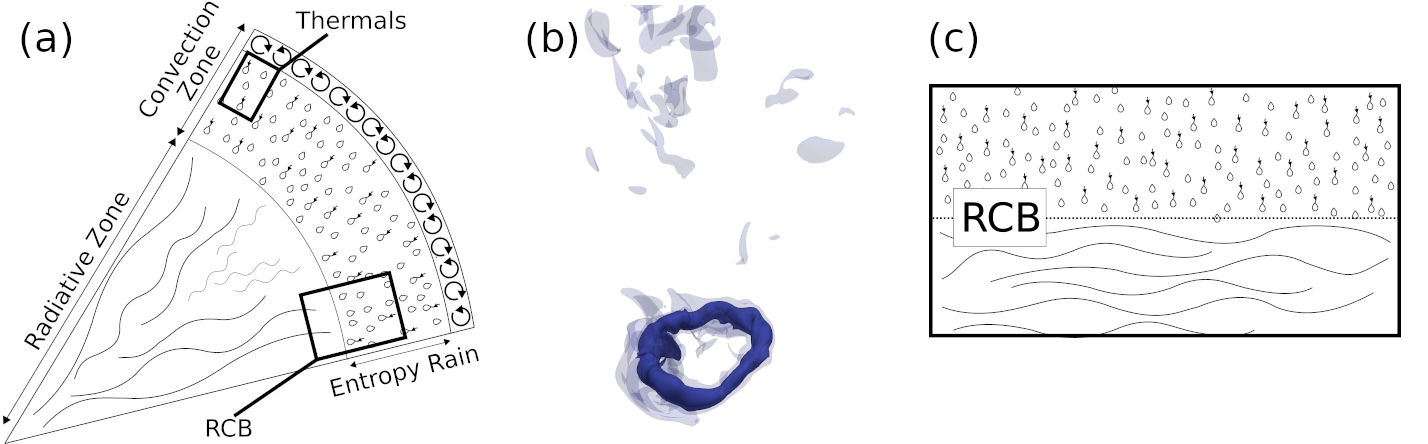
\includegraphics[width=0.9\textwidth]{./figs/tri_panel.png}
	\end{center}
    \caption{ (a) A schematic of the interior of solar-type stars under the entropy rain hypothesis, where cold droplets of fluid carry the stellar luminosity below a small traditional convective surface layer.
	The scope of the first two experiments proposed here are boxed and labeled (``Thermals'' and ``RCB'').
	(b) A 3D visualization of entropy perturbations within the downward-propagating reference frame of a turbulent thermal, which may be the dynamical form of entropy rain.
	(c) A schematic of the radiative-convective boundary (RCB), where downflows impinge upon a stable layer and excite gravity waves within that layer.
	\label{fig:tri_panel} }
	\vspace{-17pt}
\end{figure*}

\paragraph{Convection at the Smallest Scales: Individual Downflows} 
My PhD work on entropy rain and thermals \citep[][described above]{andersLB2019} neglected turbulence, magnetism, and rotation, which are key ingredients in stellar convection.
As a Princeton fellow, I will build upon my thesis work to understand if entropy rain is feasible by learning how rotation, magnetism, and turbulence affect the ability of these downflows to transit a stellar convection zone.
These physical complications could all have filtering effects on downflows, preventing their successful propagation through the stellar convection zone in certain regimes.
I will determine whether strong magnetic fields or rapid global rotation can ``evaporate'' entropy rain.
While \citet{lecoanet&jeevanjee2019} found that turbulence had little effect on the evolution of thermals in unstratified atmospheres, the compressional effects of atmospheric stratification could change this outcome, and I will explore this possibility.
Constraining the regimes in which these realistic effects prevent downflows from crossing the stellar convection zone is crucial to determining the validity of the entropy rain hypothesis.

\paragraph{Convection at the Mesoscale: Interactions at the Radiative-Convective Boundary}
In solar-type stars, the base of the convection zone is a radiative-convective boundary (RCB), where turbulent convective motions give way to a stable radiative zone.
The Sun's RCB coincides with a region of intense radial velocity shear called the tachocline, which is thought to play an important role in the solar dynamo.
Recent results suggest that the topology of a star's magnetic and angular momentum profile can affect asteroseismic measurements \citep{benomar&all2018, santos&all2018}, so it is crucial to learn the role the RCB plays in establishing these profiles.
The pumping of angular momentum and magnetism by downflows into a solar-like RCB is poorly understood.
As a Princeton fellow, I will study rotating, magnetized, time-evolving mesoscale simulations where unstable convection zones overlay stable radiative interiors, as depicted in Fig.~\ref{fig:tri_panel}c.
These simulations will be conducted in the regimes where my downflow-only thermals simulations predict that downflows are not filtered out by rotation and magnetism.
From these simulations, I will extend the work of \citet{wood&brummell2018} to determine which stellar rotation rates can create a solar-like tachocline.
Furthermore, I will study the efficiency of magnetic field pumping into the RCB to determine if RCB/tachocline interactions are one of the primary drivers of solar magnetism, as is widely believed.

\paragraph{Global Scale Convection: Dynamics in Relaxed Atmospheres}
The deficiencies of mixing length theory have led researchers to seek mechanisms which couple 1D models with fully convective, three-dimensional (3D) global simulations in order to replace convective parameterizations with sampled nonlinear statistics.
Recently, 3D spherical shell simulations of convection in thin, near-surface layers have been coupled to 1D models by \citet{jorgensen&weiss2019}.
%Unfortunately, the computational expense of 3D simulations meant that this coupling could not occur at runtime but was instead performed \emph{a posteriori}.
These near-surface simulations examine a regime where the convective overturn timescale is very similar to the local Kelvin-Helmholtz (KH) timescale of atmospheric equilibration.
In studies of deep convection, where most disagreements between simulations and observations occur \citep[the Convective Conundrum,][]{hanasoge&all2015}, these timescales become disparate, and many overturn timescales pass during one KH timescale.
As a Princeton fellow, I will extend \citet{anders&all2018} by creating and validating a generalized public module which rapidly equilibrates mean thermodynamic profiles and flows in global simulations.
I will use Dedalus, which can accurately simulate deep convective motions in global domains which include the origin at $r = 0$ \citep{lecoanet&all2019}, to test the accuracy of this tool.
This module will read in statistical measures from unequilibrated convective simulations and output the properly equilibrated mean state which can then be read back into evolving simulations.
Researchers simulating global convection using arbitrary codes will be able to use this module to rapidly equilibrate simulations with state-of-the-art turbulent dynamics.
Statistics of deep convection can be sampled from these converged states and coupled with 1D models in the same manner as \citet{jorgensen&weiss2019} coupled simulations of surface convection.
In my own research, I will employ this tool to study converged deep convection in the same dynamical regimes as my previous mesoscale studies to examine RCB interactions in a spherical geometry.
Furthermore, \citet{featherstone&hindman2016} found that rapid rotation could in some cases suppress giant cells in global simulations.
I will determine if entropy rain and rotational suppressing of giant cells can work together to explain the Convective Conundrum by seeing if giant cells are suppressed in regimes where my individual downflow studies determined that entropy rain could cross the convection zone.


\vspace{-6pt}
\section*{\textbf{Collaborative Studies at Princeton}}
Princeton University is the ideal location for me to complete this research due to the opportunities available for interdisciplinary collaborations between astrophysicists, geophysical fluid dynamicists, and applied mathematicians.
There are a number of professors within the Department of Astrophysical Sciences and at the IAS whose mentorship and collaboration I look forward to as I work on this proposed research.
Prof.~Jeremy Goodman's expertise in stellar evolution and convection, Profs.~Eve Ostriker's and James Stone's expertise in astrophysical magnetohydrodynamics, and Prof.~Adam Burrows' expertise in global convective simulations will be invaluable across all three phases of proposed research.
I am furthermore excited to collaborate with experts on convective processes in Earth's atmosphere at Princeton's Geophysical Fluid Dynamics Laboratory like Drs.~Nadir Jeevanjee and Leo Donner.
I am additionally applying for a joint Princeton-CCA Flatiron fellowship, and in my joint application to the CCA I have detailed the experts that I look forward to collaborating with in the CCA's Compact Objects and Planet Formation groups.

Princeton's postdoctoral research program would give me the freedom to study these ambitious problems in astrophysical fluid dynamics.
The projects proposed here study stellar convection from small to global scales, build naturally upon my PhD research, and help solve exciting problems in stellar structure with broad astrophysical consequences.
I look forward to the opportunity to create cross-disciplinary collaborations and to carry on Princeton's excellent research tradition while making lasting contributions towards solving the Convective Conundrum.

\vspace{-11pt}
\bibliographystyle{yahapj}
\bibliography{biblio}
\end{document}
